탐색(serach) 알고리즘은 어떤 배열에서 원하는 값이 있는지 판별하고, 있다면 몇 번째에 있는지 찾는 알고리즘을 말한다. 가장 단순한 탐색 알고리즘은 모든 배열의 값과 비교하여 $O(N)$에 탐색하는 방법이다. 이번 장에서는 $O(N)$보다 빠르게 탐색하는 방법을 배운다.

\section{빠르게 탐색하기}
다음과 같은 문제를 생각하자.
\begin{example} \label{ex: search-query}
    길이 $N$의 어떤 수열 $A$가 주어질 때, 다음과 같은 쿼리(query) $Q$개를 처리하는 프로그램을 작성하라.
    \begin{itemize}
        \item 쿼리: 수 $x_j$가 수열 $A$에 존재하면 몇 번째에 존재하는지 출력하고, 존재하지 않으면 $-1$을 출력하라.
    \end{itemize}
\end{example}

모든 수와 같은지 비교하는 완전 탐색(complete search)으로 문제를 해결할 경우 $O(NQ)$의 시간이 걸릴 것이다. 하지만 만약 배열이 정렬되어 있다면 어떨까? 우리는 다음 관찰이 성립함을 확인할 수 있다.

\begin{obs}
    $k$번째 값보다 원하는 값 $x_j$가 크면 $i<k$번째 값은 확인할 필요가 없고, 작으면 $i>k$번째 값은 확인할 필요가 없다.
\end{obs}

이분 탐색(binary search)의 아이디어는 이 관찰로부터 비롯된다. 만약 $k$를 $x_j$가 있을 가능성이 있는 범위의 중간 지점으로 잡는다면, 한 번의 비교로 구간의 길이를 절반으로 줄일 수 있고, 적어도 $O(\log N)$번 안에 탐색을 완료할 수 있다.

이를 쉽게 이해하기 위해 up-down 게임을 생각해보라. up-down 게임은 술래가 $100$ 이하의 숫자 $x$를 생각하면 다른 플레이어가 숫자 $y$를 말해 $x>y$이면 down, $x<y$이면 up이라고 말해주는 게임이다. 이 게임에서 최적 전략은 무엇일까? 당연히 처음에 $50$을 물어보고 답을 들을 것이다. 왜냐하면 up이라는 대답을 들어도, down이라는 대답을 들어도 남는 숫자의 개수가 가장 작은 숫자가 중간값인 $50$이기 때문이다. 여러분은 이미 이분 탐색을 사용하고 있다!

(누군가는 $10$을 물었을 때 down이라는 대답을 들으면 더 빨리 수를 찾는 것 아니냐고 말하기도 한다. 하지만 반대로 생각해보라. 만약 up이라는 대답을 들었다면 아직도 $90$개의 숫자가 가능한 후보이다. Problem Solving에서는 항상 최악 시간복잡도를 생각해야 한다는 사실을 잊지 말자.)

이제 이분 탐색을 구현을 해보자. 우리는 가능한 구간의 시작과 끝을 나타내는 변수 \texttt{st, ed}를 선언해야 한다. 그리고 그 중간 위치 \texttt{mid}와 현재 값을 비교해 구간을 줄이면 된다. 구현은 \Cref{code: binary-search}을 참고하라.

\begin{code} \label{code: binary-search}
이분 탐색 알고리즘
\begin{lstlisting}
void binary_search(int x) {
    int x, ans = -1;
    cin >> x;
    int st = 1, ed = n;
    while (st < ed) {
        int mid = (st + ed) / 2;
        if (x == arr[mid]) {
            ans = mid;
            break;
        }
        if (x < arr[mid]) ed = mid - 1;
        if (x > arr[mid]) st = mid + 1;
    }
    cout << ans << "\n";
}
\end{lstlisting}
\end{code}

\texttt{while}문 하나로도 해결할 수 있을 정도로 알고리즘은 매우 단순하다. 하지만 이분 탐색은 수많은 문제에서 쓰이는 아주 중요한 알고리즘이므로 꼭 숙지하도록 하자.

\section{STL 내장 함수}
이분 탐색은 사용되는 경우가 매우 많기 때문에 STL에서 내장 함수로 지원한다. 두 종류의 함수 \texttt{std::lower\_bound(start, end, value)}와 \texttt{std::upper\_bound(start, end, value)}가 있다. 각각의 함수는 다음을 반환한다.

\begin{itemize}
    \item \texttt{std::lower\_bound(start, end, value)}: $[\texttt{start}, \texttt{end})$에서 \texttt{value} 이상인 가장 앞의 수를 가리키는 포인터를 리턴한다. 없으면 \texttt{end}를 리턴한다.
    \item \texttt{std::upper\_bound(start, end, value)}: $[\texttt{start}, \texttt{end})$에서 \texttt{value} 초과인 가장 앞의 수를 가리키는 포인터를 리턴한다. 없으면 \texttt{end}를 리턴한다.
\end{itemize}

\texttt{std::sort}와 다르게 \texttt{compare} 인자가 없다. 즉, 비교 기준을 임의로 설정할 수 없다. 만약 다른 비교 기준이 필요하다면 이상과 초과는 \texttt{<} 연산자를 바탕으로 판단하므로 연산자 오버로딩을 사용하라.

다음 \Cref{code: lower_bound}와 \Cref{code: upper_bound}은 cppreference.com에서 제공하는 예시 코드이다. 예시 코드를 보고 사용방법을 숙지하자.

\begin{code} \label{code: lower_bound}
\texttt{std::lower\_bound} 예시 코드: \url{https://en.cppreference.com/w/cpp/algorithm/lower_bound}
\begin{lstlisting}
#include <algorithm>
#include <iostream>
#include <vector>
    
struct PriceInfo { double price; };
    
int main()
{
    const std::vector<int> data{1, 2, 4, 5, 5, 6};
    
    for (int i = 0; i < 8; ++i)
    {
        
        auto lower = std::lower_bound(data.begin(), data.end(), i);
    
        std::cout << i << " <= ";
        lower != data.end()
            ? std::cout << *lower << " at index " << std::distance(data.begin(), lower)
            : std::cout << "not found";
        std::cout << '\n';
    }
    
    std::vector<PriceInfo> prices{{100.0}, {101.5}, {102.5}, {102.5}, {107.3}};
    
    for (double to_find : {102.5, 110.2})
    {
        auto prc_info = std::lower_bound(prices.begin(), prices.end(), to_find,
            [](const PriceInfo& info, double value)
            {
                return info.price < value;
            });
    
        prc_info != prices.end()
            ? std::cout << prc_info->price << " at index " << prc_info - prices.begin()
            : std::cout << to_find << " not found";
        std::cout << '\n';
    }
}
\end{lstlisting}
\end{code}

\begin{code} \label{code: upper_bound}
\texttt{std::upper\_bound} 예시 코드: \url{https://en.cppreference.com/w/cpp/algorithm/upper_bound}
\begin{lstlisting}
#include <algorithm>
#include <iostream>
#include <vector>
    
struct PriceInfo { double price; };
    
int main()
{
    const std::vector<int> data{1, 2, 4, 5, 5, 6};
    
    for (int i = 0; i < 7; ++i)
    {
        // Search first element that is greater than i
        auto upper = std::upper_bound(data.begin(), data.end(), i);
    
        std::cout << i << " < ";
        upper != data.end()
            ? std::cout << *upper << " at index " << std::distance(data.begin(), upper)
            : std::cout << "not found";
        std::cout << '\n';
    }
    
    std::vector<PriceInfo> prices{{100.0}, {101.5}, {102.5}, {102.5}, {107.3}};
    
    for (double to_find : {102.5, 110.2})
    {
        auto prc_info = std::upper_bound(prices.begin(), prices.end(), to_find,
            [](double value, const PriceInfo& info)
            {
                return value < info.price;
            });
    
        prc_info != prices.end()
            ? std::cout << prc_info->price << " at index " << prc_info - prices.begin()
            : std::cout << to_find << " not found";
        std::cout << '\n';
    }
}
\end{lstlisting}
\end{code}

\section{연습문제 A}
\begin{problem}
    완전 탐색으로 \Cref{ex: search-query}을 해결하는 코드를 작성하라.
\end{problem}
\begin{problem}
    이분 탐색으로 \Cref{ex: search-query}을 해결하는 코드를 작성하라. 시간복잡도는 무엇인가?
\end{problem}
\begin{problem}
    STL 내장 함수를 이용해 \Cref{ex: search-query}을 해결하는 코드를 작성하라.
\end{problem}

\section{연습문제 B}

\begin{problem}
    (17124번) 길이 $N$의 배열 $A$와 길이 $M$의 배열 $B$로 길이 $N$의 배열 $C$를 만드려고 한다. $C_i$는 $B$에 있는 수들 중 $A_i$와의 차이가 가장 작은 수이다. 만약 이러한 수가 여러 개라면 크기가 가장 작은 수를 고른다. $\sum_{i=1}^N C_i$를 구하여라. $N \leq 10^6$, $M \leq 10^6$이다.
\end{problem}

\begin{problem}
    (19554번) $X \in [!, N]$인 $X$를 찾아라. \textbf{단, 이 문제는 인터랙티브 문제로 입출력을 통해 채점 프로그램과 소통해야 한다.}
    \begin{itemize}
        \item $P$를 출력하여 질의한다. 그러면
        \item 채점 프로그램은 $P < X$이면 \texttt{-1}을 출력한다.
        \item 채점 프로그램은 $P = X$이면 \texttt{0}을 출력하고 프로그램을 종료한다.
        \item 채점 프로그램은 $P > X$이면 \texttt{1}을 출력한다.
    \end{itemize}
    $N \leq 10^9$이며 질의 횟수는 50회 이하여야 한다. (hint. 첫 번째 인터랙티브 문제이다. 직접 제출하여 채점해보라. \texttt{cout << flush}로 버퍼를 비우는 것을 잊지 말자.)
\end{problem}

\begin{problem}
    (1056번*) 다음 세 연산으로 $N$을 만들기 위해 필요한 최소 연산 횟수를 출력하라. $N \leq 10^{18}$이다.
    \begin{itemize}
        \item $N \rightarrow N+1$
        \item $N \rightarrow N-1$, $N > 1$
        \item $N \rightarrow N^x$, $x$는 자연수
    \end{itemize}
\end{problem}

\begin{problem}
    (1208번*) $N$개의 정수로 이루어진 수열에서 몇 개를 골라 다 더한 값이 $S$가 되는 경우의 수를 구하여라. $N \leq 40$이고 수열의 값은 절댓값이 $10^5$ 이하인 정수, $S$는 절댓값이 $10^6$ 이하인 정수이다.
\end{problem}

\begin{problem}
    (5631번) $N$개의 점의 집합 $S$와 두 점 $(a_x, a_y)$와 $(b_x, b_y)$가 주어질 때 다음 쿼리 $Q$개를 처리하는 프로그램을 작성하라. $N \leq 2 \cdot 10^5$, $Q \leq 20000$, 모든 점의 좌표는 $20000$ 이하의 음 아닌 정수이다.
    \begin{itemize}
        \item 입력으로 주어지는 $R_1$과 $R_2$에 대하여 $(a_x, a_y)$가 중심이고 반지름이 $R_1$인 원에 속하는 $S$의 원소의 개수와 $(b_x, b_y)$가 중심이고 반지름이 $R_2$인 원에 속하는 $S$의 원소의 개수의 합을 출력하라. $R_1$과 $R_2$는 모두 $13000$ 이하의 자연수이다.
    \end{itemize}
\end{problem}

\begin{problem}
    (10425번) 주어진 21000자리 이하의 피보나지 수가 몇 번째 피보나치 수인지 출력하라. 피보나치 수의 점화식은 아래를 참고하라. 답이 $10^5$ 이하임이 보장된다.
    $$F_n = \begin{cases} 0 & n=0 \\ 1 & n=1 \\ F_{n-1} + F_{n-2} & n>1 \end{cases}$$
\end{problem}

\begin{problem}
    (15425번*) 순서대로 $1$번부터 $N$번까지 번호가 붙어 있는 $N$개의 고층 빌딩이 있다. 각 고층 빌딩의 높이는 $H_i$이고 고층 빌딩에서 얻을 수 있는 금화의 개수는 $G_i$이다. 여러분은 다음 조건을 만족하도록 몇 개의 빌딩을 순서 없이 고를 수 있다. 
    \begin{itemize}
        \item 고른 빌딩을 번호가 증가하도록 나열하면 높이가 단조증가해야 한다.
        \item 고른 빌딩에 있는 금화의 개수의 합은 $K$ 이상이어야 한다.
    \end{itemize}
    위 조건을 만족하도록 고층 빌딩을 고르는 경우의 수를 출력하라. $N \leq 40$, $H_i \leq 10^9$, $G_i \leq 10^9$이다.
\end{problem}

\begin{problem}
    (22882번*) 정수로만 이루어진 $N \times N$의 이차원 배열에서 1행 1열에서 $N$행 $N$열까지 최단거리로 이동하는 경로를 하나 골라 길이 $2N-1$의 수열 $a_k$를 만드려고 한다. 이러한 과정으로 만들어지는 수열 중
    $$\max_{1 \leq i \leq j \leq 2N-1} \left(\sum_{k=i}^j a_k\right)$$
    의 값이 $K$인 수열의 개수를 출력하라. $N \leq 20$이고 이차원 배열에 적힌 수는 절댓값이 $10^9$ 이하인 정수이다.
\end{problem}

\begin{problem}
    (24047번*) 길이 $N$의 배열을 버블 정렬로 오름차순 정렬하는 아래 의사 코드를 참고하여 $K$번 교환 후 배열을 출력하라. $K$번 교환 전에 정렬이 완료된다면 $-1$을 출력하라. $N \leq 5 \cdot 10^5$, $K \leq 10^8$이고 배열의 각 원소는 $10^9$ 이하의 자연수이다.
    
    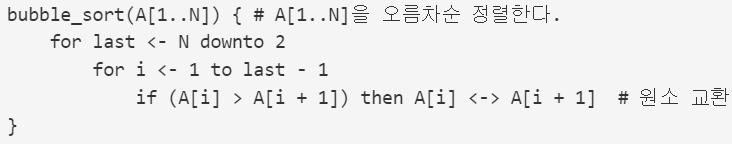
\includegraphics[width=0.8\textwidth]{Images/24074.png}
\end{problem}

\section{연습문제 C}
\begin{problem}
    (20084번) 숨겨진 길이 $N$의 바이너리 문자열 $T$가 있다. 여러분은 $S$가 $T$의 연속 부분문자열인지 판단하는 질의를 $t$번 이내로 사용하여 $T$를 알아내어야 한다.
    \begin{itemize}
        \item (서브테스크 1) $N \leq 5$, $t = 31$
        \item (서브테스크 2) $N \leq 100$, $t = 256$
        \item (서브테스크 3) $N \leq 1000$, $t = 1024$
    \end{itemize}
\end{problem}
